% ==================================================================
%  Time lapse of the flight -- one sigconf text width, pdfLaTeX
%  Preamble:  \usepackage{tikz}  (graphicx comes with acmart);
%             flight-strobe.png on the graphics path
%  Image:     flight-strobe.png (8.20 x 5.28 cm, 600 dpi), made by
%             cpp2lean sim/figs/render_strobe.py: copter_lean (the Lean
%             translations of ArduPilot's classes, lean/.lake/build/bin/copter_lean)
%             re-flying the figure-eight course of sim/params/copter-cf2x.txt at
%             1 m/s (copter-course-speed.txt) with the tuned gains
%             (copter-cf2x-tuned.txt) headless through sim/run_copter.py's fly
%             (400 Hz control, 1200 Hz physics, 7797 ticks); the vehicle pose
%             taken every 0.5 s from t = 0.6425 s (the first instant
%             5 cm above the start) to 16.1425 s, plus one instant at the
%             final hover (t = 19.4875 s), 33 in all, and rendered by PyBullet
%             (getCameraImage, ER_TINY_RENDERER, 4x supersampled) from one fixed
%             oblique camera (yaw 22, pitch -34, distance 10.2 m);
%             vehicle pixels found by differencing against the empty scene and
%             composited with opacity rising toward the last instant. The
%             vehicle mesh is drawn at 3 times its size. The re-flown actuator
%             and state lines equal those of the recorded flights
%               motors.txt vs sim/out/lean-course-1ms/motors.txt: 7797 vs 7797 lines, 0 differ
%               inputs.txt vs sim/out/lean-course-1ms/inputs.txt: 7797 vs 7797 lines, 0 differ
%               motors.txt vs sim/out/ref-course-1ms/motors.txt: 7797 vs 7797 lines, 0 differ
%               inputs.txt vs sim/out/ref-course-1ms/inputs.txt: 7797 vs 7797 lines, 0 differ
%             No text in the image; labels sit beside the projected vehicle
%             centers written by the script to sim/figs/out/strobe/labels.txt,
%             at the first instant, the instant nearest each inner waypoint's
%             closest approach (summary.txt), and the final hover (with the
%             last course instant when the two are within a tenth of the image
%             width), each on the side away from the waypoints' centroid.
%             Generated by the script; no hand-edited coordinates.
% ==================================================================
\definecolor{fwInk}{HTML}{22252A}%
\definecolor{fwMute}{HTML}{8A8F96}%
\begin{tikzpicture}[tl/.style={font=\scriptsize, text=fwMute, inner sep=0.5pt}]
\node[anchor=south west, inner sep=0] (img) at (0,0)
  {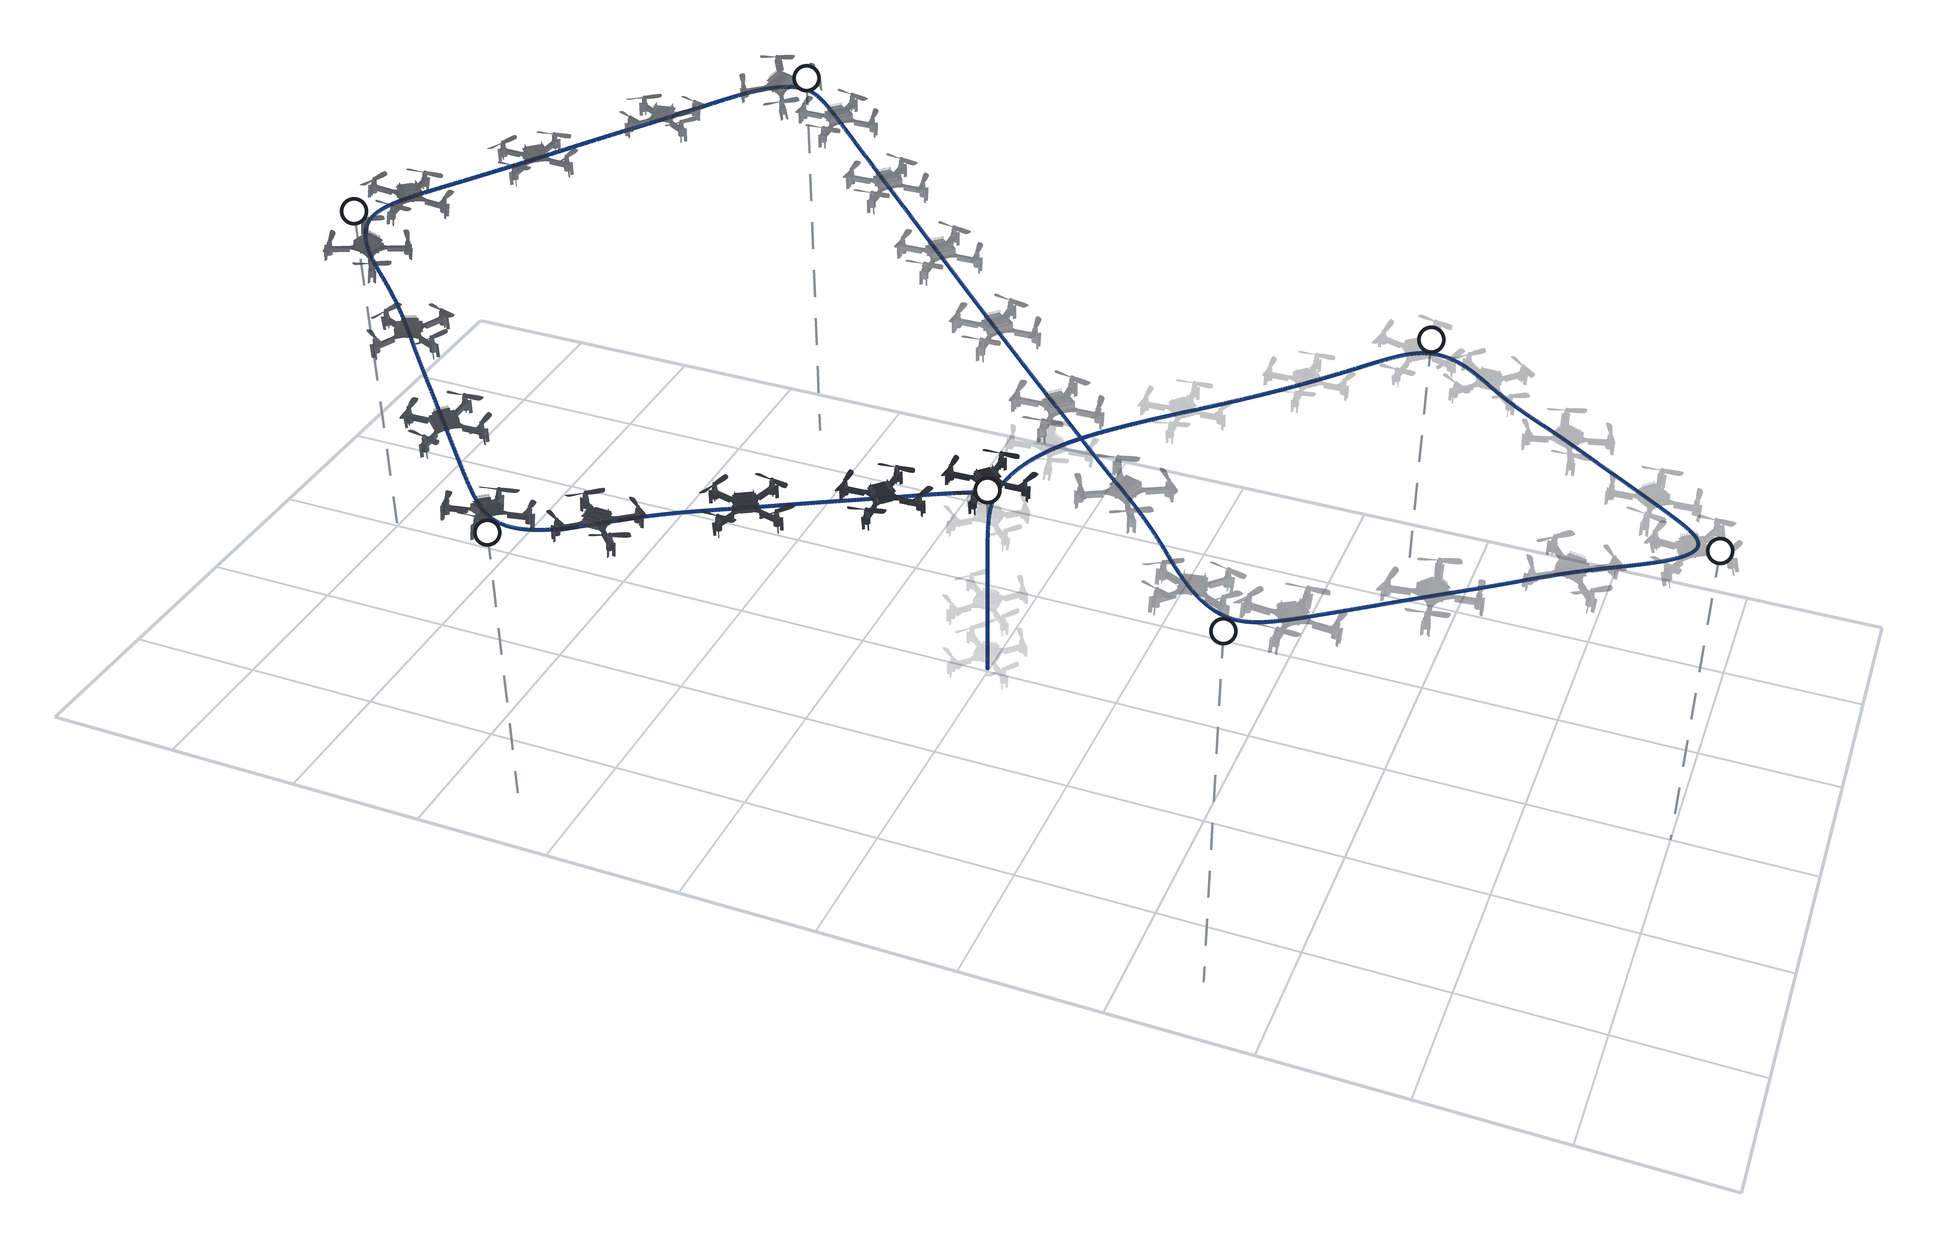
\includegraphics[width=\linewidth]{flight-strobe.png}};
\begin{scope}[x={(img.south east)}, y={(img.north west)}]
  \node[tl, anchor=north] at (0.509,0.427) {$t=0.6$\,s};
  \node[tl, anchor=west] at (0.760,0.727) {3.6\,s};
  \node[tl, anchor=west] at (0.902,0.544) {5.6\,s};
  \node[tl, anchor=north west] at (0.633,0.488) {7.6\,s};
  \node[tl, anchor=south east] at (0.392,0.973) {11.1\,s};
  \node[tl, anchor=south east] at (0.185,0.865) {12.6\,s};
  \node[tl, anchor=east] at (0.222,0.575) {14.6\,s};
  \node[tl, anchor=north east] at (0.435,0.567) {16.1, 19.5\,s};
\end{scope}
\end{tikzpicture}%
